% useful links

% Notion (Aufgabenboard):
% https://app.notion.com/p/Teamspace-Startseite-792cfed96e0d838b930c01feb08adf30?source=copy_link

% LaTeX:
% https://sharelatex.tu-darmstadt.de/6146834165krbsdbsngyjt#763634

% GitHub Repo:
% https://github.com/sxndrx-cxlxnx/TU_Computing_4_Social_Good

% Figma Design Projekt:
% https://www.figma.com/design/vKBOiex8tUQbbK5JqksHRP/Comp4SG---TheMissingAdult?node-id=0-1&m=dev&t=IILaY3qqmfAZ6BlI-1

% Kommunikation: WhatsApp + Discord


\documentclass[
	ngerman,% Main language as global option
	accentcolor=9c,% Choose accent color: For a list of available colors see the full tudapub documentation
	type=intern, % Minimal setup without accent color
	marginpar=false,% Disable marginpar
    parskip=half,% Absätze mit Abstand statt Einzug
%	accept-missing-logoes=true,% No error in case logo files are not available
%	logofile=example-image,% In case logo should be replaced
    logofile=media/tuda_logo.png
]{tudapub}

\usepackage[ngerman]{babel}
\usepackage[autostyle]{csquotes}% \enquote, to simplify use of quotation marks
\usepackage{tabularx}
\usepackage{booktabs} % Für professionelle Linien (\toprule, \midrule, \bottomrule)

\usepackage[backend=biber]{biblatex}
\addbibresource{references.bib}
\title{Team 3 - TheMissingAdult}
\subtitle{It takes a village to raise a child.}
\author{Umut B. Aktas, Sude Avara, Zhaneta Gasparyan, Simona Georgieva, Sandra Gräf, Anna Trutneva}
\date{DD.MM.YYYY}

\begin{document}

\maketitle

\tableofcontents
% Additional lists like \listoffigures or acronyms might be added here

%\enquote{DEMO-TUDaReport.tex} is a minimal template for using the document class \enquote{tudapub.cls}. It is part of TUDa-CI, which is the official template bundle of TU Darmstadt. The original version was inspired by the \enquote{tuddesign} bundle by C.~v.~Loewenich and J.~Werner.

\section{Template Instructions}
Disclaimer: This template serves as a structured guide for your report. While the format and sections provided offer a framework, you have  creative freedom to adapt and modify the template to best suit your project and presentation style. 

The key requirement is ensuring all necessary information and core design  elements are included in your final submission. Feel free to reorganize sections, adjust the layout, incorporate visual elements, or present your findings in whatever format best communicates your design process and outcomes. Think of this as a starting point rather than a rigid structure. 

% use \input for including without pagebreak

% Design
\section{Motivation}
\emph{Why should we care about your idea?}

\begin{itemize}
    \item Start with compelling statistics, news article, or research finding that establishes the problem's scope: \emph{What would happen if this problem continues unsolved?}
    \item Connect your problem to current trends or overarching themes (DEI, sustainability, mental health, etc.): \emph{What recent events or trends make this problem more urgent?}
    \item Include a brief personal anecdote or observation that motivated your team: \emph{What personal experience connects your team to this issue?}
    \item If possible, quantify the impact: How many people face this problem? How much time/money/effort/\textbf{pain} does it cost them? This does not mean it needs to benefit all humankind, small scale interventions are more than welcome!
\end{itemize}
\section{Overview}
\emph{Our application allows users to [primary action] and [secondary action] through [key method], enabling them to [desired outcome] instead of [current frustration].}

\begin{itemize}
    \item Problem statement: One clear sentence defining exactly what problem you are solving. \emph{[Specific user group] struggles with [specific challenge] because [root cause].}
    \item Target user profile: Context use and specific demographics (age range, education, geographic location), behaviors, and needs (including accessibility needs, physical, cognitive, economic barriers). \emph{Our primary users are [detailed description including age, lifestyle, tech comfort, constraints].}
    \item Solution description: What your app does in 2-3 sentences, focusing on user actions, not features. \emph{Our app allows users to [primary action] and [secondary action] through [key method].}
    \item Key differentiator: How your solution is different from existing options. Research existing solutions and identify what they do well, what they miss, how your approach is different, why your solution is needed despite existing options. \emph{Unlike [existing alternatives], our solution [unique approach or benefit].}
    \item Explicitly connect your solution to (loosely) at least one UN Sustainable Development Goal and explain how your app contributes to positive social change.
\end{itemize}
\section{Design Thinking - 1. Draft}
\emph{How and why did we use Design Thinking?}

\begin{itemize}
    \item Detailed interview methodology: How you recruited participants (social media, personal, etc.), interview duration, recording of interviews, location, incentives offered
    \item Participant demographics: Age ranges, study programs, habits, tech usage patterns
    \item Critical reflection: Honest assessment of design thinking's limitations in your project
    \item Process challenges: What didn't work as expected and how you adapted
\end{itemize}

1. Unsere Projektidee

Mit unserer App möchten wir alleinerziehende Eltern unterstützen, die hauptsächlich für die Betreuung eines Kindes verantwortlich sind. Im Alltag kann es immer wieder passieren, dass Eltern plötzlich verhindert sind. Vielleicht müssen sie unerwartet ins Krankenhaus, haben einen dringenden Termin oder können ihr Kind aus einem anderen Grund nicht rechtzeitig abholen. Besonders für Alleinerziehende kann das schwierig werden, wenn keine zweite Betreuungsperson zur Verfügung steht.

Unsere Idee ist deshalb eine App, mit der Eltern schon im Voraus einen kleinen Kreis aus vertrauten Personen zusammenstellen können. Das könnten zum Beispiel Familienmitglieder, Freunde oder Nachbarn sein. Wenn sie keine Möglichkeit haben geben wir auch die Option  zur Betreuungsagentur yu bitten. Falls kurzfristig Hilfe benötigt wird, sollen diese Personen möglichst schnell informiert werden.

Außerdem können Eltern wichtige Informationen über die Betreuung ihres Kindes hinterlegen, damit die helfende Person weiß, worauf sie achten muss.

Unser Ziel ist es, die Zusammenarbeit zwischen Menschen zu erleichtern, die sich bereits kennen und gegenseitig vertrauen. Im Mittelpunkt stehen dabei drei Dinge: Vertrauen, Sicherheit und gegenseitige Unterstützung.

% ***************************************************************
%           User Persona
% ***************************************************************
\subsection{User Persona}
\emph{Include Activity of Persona.}

Follow the template provided or from the internet to include a visual persona with picture, demographics, goals, frustrations, and technology habits. Base everything on discussions with your team and interviews, this is an iterative approach. Create 1 to 3 primary personas maximum, depending on your target group.

% ***************************************************************
%           Define
% ***************************************************************
\subsection{Define}
\emph{Include Activity of Problem Definition.}


\textbf{Probleme und Bedürfnisse von Alleinerziehenden}

\begin{itemize}
    \item Notfallsituationen
    \begin{itemize}
        \item Elternteil wird plötzlich krank, z.B. Elternteil hat einen Unfall
        \item Unerwarteter Krankenhausaufenthalt
        \item Kind kann nicht rechtzeitig von der Kita oder Schule abgeholt werden
        \item Elternteil hat einen dringenden Termin
        \item Unerwartete Verspätung
        \item Elternteil ist vorübergehend nicht erreichbar
        \item Bereits organisierte Kinderbetreuung fällt kurzfristig aus
    \end{itemize}
    
    \item Bedürfnisse von Alleinerziehenden
    \begin{itemize}
        \item Schnelle und zuverlässige Unterstützung im Notfall-Einfache und direkte Kommunikation
        \item Vertrauenswürdige und autorisierte Betreuungspersonen
        \item Möglichkeit, eine bevorzugte Betreuungsperson auszuwählen
        \item Schnelle Organisation einer Kinderbetreuung
        \item Klare Informationen zur Abholung und Übergabe des Kindes
        \item Sichere Weitergabe wichtiger Informationen über das Kind
        \item Alternative Betreuungsmöglichkeiten, wenn Familie oder Freunde nicht verfügbar sind
        \item Sicherheit und Kontrolle über die Betreuung des Kindes
    \end{itemize}
\end{itemize}

\textbf{App-Funktionen und Ideen}

\begin{itemize}
    \item Notfallfunktion
    \begin{itemize}
        \item Notfallnachricht so schnell wie möglich senden
        \item Auswahl von Betreuungspersonen - Familienmitglieder, Verwandte, Freunde oder Betreungsagentur(z.B Nannys, Leihomas) 
    \end{itemize}
    
    \item Betreuungspersonen
    \begin{itemize}
        \item Bevorzugte Person festlegen
        \item Bei mehreren Zusagen Betreuungsperson auswählen
    \end{itemize}
    
    \item Betreuungsinformationen
    \begin{itemize}
        \item Kurze Fragen (Ja/Nein, Auswahl oder Freitext)
        \item Wo soll das Kind abgeholt werden?→ Wohin soll das Kind gebracht werden? (eigenes Zuhause / Betreuungsperson)
        \item Bis wie viel Uhr wird Betreuung benötigt?
        \item Feld für zusätzliche Anmerkungen
    \end{itemize}
    
    \item Gesundheit des Kindes
    \begin{itemize}
        \item Ist das Kind krank? (Ja/Nein)
        \item Angaben zu Krankheit und Medikamenten
        \item Hinweise zur Medikamenteneinnahme
    \end{itemize}
\end{itemize}

\textbf{1. Skizze - Layout}

\begin{figure}[h]
    \centering
    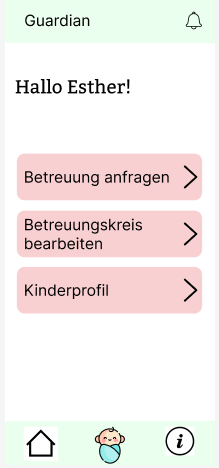
\includegraphics[width=0.2\linewidth]{media/Eltern-Startseite-1.draft.png}
    \caption{Startseite - Elternprofil (1. Draft)}
    \label{fig:1.Draft:Eltern:Startseite}
\end{figure}

% ---------------------------------------------------------------
% ------------- BEGIN TABLE -------------------------------------
% ---------------------------------------------------------------
\newpage
\textbf{1. Skizze - Funktionale Inhalte}
% Please add the following required packages to your document preamble:
% \usepackage{tabularx}
\begin{table}[h]
\centering
\begin{tabularx}{\linewidth}{|l|X|X|X|}
\hline
    & Startseite  & Betreuungsseite  & Profil  \\ \hline
                 
Eltern
& - Appname\newline - Notification-Symbol\newline - 3-4 Buttons = Shortcuts zu:\newline $\rightarrow$  Betreuungsanfrage stellen\newline $\rightarrow$ Betreuungskreis bearbeiten\newline $\rightarrow$ Kinder-Informationen bearbeiten
& Aktive Anfrage:\newline - Wer soll die Betreuung übernehmen\newline $\rightarrow$ vertraute Person oder Betreuungsagentur wählen\newline - Betreuungsdetails bearbeiten (Wann, Abholung, Betreuungsort, Gesundheit, Zusätzliche Hinweise)
& - hier: Kinderprofil\newline - Bearbeiten-Knopf einfügen\newline - allgmein: Name, Altern, Bild\newline - medizinische Informationen: Medikamente, Ärute / Hausarzt\newline - Kontakt: Adresse, Notfallkontakt (Telefonnummern) der der Eltern\newline - Einstellungen (Benachrichtigung, Datenschutz)                                                                                                         \\ \hline

Betreuungsperson
& - Appname\newline - Notification-Symbol\newline - Hallo {[}Name{]}\newline - 3-4 Buttons\newline $\rightarrow$ Neue Anfragen\newline $\rightarrow$ Betreuungskreise (Familien, die dich eingeladen haben)\newline $\rightarrow$ Mein Profil
& Anfrage:\newline - Status: Neu, Angenommen, Offen, Vergangen / Abgeschlossen\newline - Betreuungsdetails einsehen (Kindsname, Wann, Abholung, Betreuungsort, Gesundheit, Wichtige Hinweise)\newline - Button - Betreuung zusagen / Ablehnen
& - hier: Profil der BP\newline - Bearbeitenknopf einfügen\newline - Meine Verfügbarkeit (Zeiten festlegen)\newline - angebotene Dienstleistungen\newline $\rightarrow$ aus denen Eltern die zugetrauten Berechtigungen ableiten / auswählen können\newline $\rightarrow$  z.B. Betreuung bei sich oder bei Eltern, Abholen ja/nein, Arztbesuche ja/nein etc.\newline - Einstellungen (Benachrichtigung, Datenschutz)\\ \hline
\end{tabularx}
\end{table}
% ---------------------------------------------------------------
% ------------- END TABLE ---------------------------------------
% ---------------------------------------------------------------


% ***************************************************************
%           Ideate
% ***************************************************************
\subsection{Ideate}
\emph{Include Activity of Ideation Process.}

% ***************************************************************
%           Critical Reflection
% ***************************************************************
\subsection{Critical Reflection on Design Thinking}

\begin{itemize}
    \item What worked well with this approach for your project?
    \item What challenges did you encounter? (time constraints, participant recruitment, conflicting feedback)
    \item When did design thinking not provide clear direction?
    \item What alternative approaches might have been more effective?
\end{itemize}
\section{Requirements}
\emph{Show your learning journey through changing requirements.}

Format as stages with clear triggers (The following only serves as an example).
\begin{itemize}
    \item Stage 1: Initial Requirements (Week 1-2). Based on team assumptions and initial research. List core features you initially planned (functional 'what the app does' and non-functional requirements such as usability, accessibility standards). You can use user stories \emph{As a [user type], I want [functionality] so that [benefit]}. 
    \item Stage 2: Post-Interview Requirements (Week 3-4). Based now on user interviews and persona development. Document what changed, e.g. specific requirements that were modified, added, or removed, and also why it changed and how these changes affected your overall solution approach.
    \item Stage 3: Post-Prototype Requirements (Week 5-6). This is now based on usability testing and iterative feedback, where you refine your requirements, resulting in a final list of must-have features.
\end{itemize}
\section{Design}

\begin{itemize}
    \item Evolution timeline: Visual progression from paper sketches to final digital prototype
    \item Iteration triggers: What specific feedback or insight led to each major change
    \item Usability testing results: Document what users struggled with and how you responded
    \item Design decisions: Explain why you chose specific layouts, navigation patterns, or visual elements
    \item Abandoned concepts: Show designs you tried but rejected, with explanations
\end{itemize}

% ***************************************************************
%           Mockups / Low-Fi Prototype
% ***************************************************************
\subsection{Mockups/Low-Fi Prototype}

\begin{itemize}
    \item Iteration 1: Paper Sketches (Week 1): [Include photos of hand-drawn wireframes], Basic Layout, Navigation
    \item Iteration 2: Digital Wireframes (Week 3):
[Include Figma/Sketch screenshots], Changes
    \item Usability testing results: Document what users struggled with and how you responded
    \item ...
\end{itemize}

% ***************************************************************
%           MLP / High-Fi Prototype
% ***************************************************************
\subsection{MLP/High-Fi Prototype}
\emph{From Initial Prototype To Final MLP}

\begin{itemize}
    \item What specific actions did you ask users to perform?
    \item What did users struggle with? What worked well?
    \item Justify your Visual Design Decisions such as color choices and accessibility considerations, typography and readability, icon selection and cultural sensitivity. Take care of Accessibility Features such as color contrast ratios, text size and scalability, navigation for screen readers, alternative input methods!
\end{itemize}

\section{Architecture}
\emph{Technical foundation for your application.}

\begin{itemize}
    \item Platform justification: Explain why you chose web app vs mobile app vs desktop based on user research
    \item System components diagram: Visual representation of how different parts of your app connect
    \item Data architecture: What information your app handles and how it is organized
    \item User flow documentation: Step-by-step paths users take through your app
    \item Integration requirements: External services your app would need (APIs, databases, authentication)
    \item Scalability considerations: How your architecture would handle growth
\end{itemize}

% surroundings
\section{Risk Management}
\begin{itemize}
    \item Technical risks: What could go wrong with your prototype or future implementation (e.g., API changes, older devices)?
    \item User adoption risks: Why users might not adopt or continue using your solution (e.g., maintainance of real-time information)? Why might users be hesitant to try your solution?
    \item Business/project risks: External factors that could impact success (e.g., political changes)
    \item Mitigation strategies: Specific actions to reduce or eliminate each risk
    \item Social/Ethical Risks: What if your users cannot access or afford the technology? What if users struggle with technology? How do you ensure your solution respects cultural differences? How might your solution accidentally harm your target population? Could users become unhealthily dependent on your app?
\end{itemize}
\section{Legal and Ethical Considerations}
\begin{itemize}
    \item Data privacy requirements: What user data you collect and how you protect it
    \item Vulnerable Population Protections: If your app serves minors, elderly, or other vulnerable groups?
    \item Accessibility compliance: Legal requirements for inclusive design
    \item Intellectual property: Patents, trademarks, or copyrights that might affect your solution
    \item Platform compliance: App store policies or web accessibility standards
\end{itemize}
\section{Social Impact Assessment}
\emph{This is a new section specifically for social good applications since we discussed a lot about the definition of social good.}

\begin{itemize}
    \item What constitutes success vs. failure? What quantitative and qualitative measures do you have? How will you measure social impact?
    \item How will you capture user transformation narratives?What behavioral changes will you observe?
    \item How will your solution continue to create social good without your team? What partnerships or funding would be needed?
    \item How will you ensure long-term user engagement? versus What would happen if the app stopped working tomorrow?
\end{itemize}
\section{Team Reflections}
\emph{Weekly honest reflections (250 words each week) as a team.}

Write about 250 words as a team each week on what you have experienced this week and what you have learned.
This should always be on Monday or Friday. Be honest, it is okay if things did not work out---it is important to learn from those experiences.

% ***************************************************************
%           Week 1
% ***************************************************************
\subsection{Week 1: 15.05 or 19.05}
\emph{Write about everything that is going on in your team. Go beyond the actual facts: How have you felt this week? Confident? Anxious? Frustrated? Excited? Motivated? Happy? ... And WHY?}

\begin{itemize}
    \item What you accomplished as a team such as specific tasks completed, milestones reached, decisions made
    \item What you learned about our users, problem, solution, working as a team
    \item The challenges faced, successes and failures (and why they happened)
    \item Your emotional journey as how did team members feel, what caused these feelings, how did emotions affect your work?
\end{itemize}

% ***************************************************************
%           Week 2
% ***************************************************************
\subsection{Week 2: 23.05 or 26.05}
...

% ***************************************************************
%           Week 3
% ***************************************************************
\subsection{Week 3:}
...

\section{Key Learnings}
\emph{For your final submission: Reflection on your journey throughout the semester.}

\begin{itemize}
    \item What we assumed: Specific belief you held initially
    \item What we discovered: Contradictory evidence from user research
    \item Process insights: What worked well in your team dynamics and what created friction
    \item Impact on our solution: How this changed your approach
    \item Lesson learned: What this taught you about user research/design/software development
    \item Skill Development Documentation: New skills gained such as specific abilities developed (interviewing, creativity, teamwork, prototyping, etc.), and how you acquired new skills. 
    \item Reflect on your team dynamics: What collaboration patterns worked well? What caused friction and how did you resolve it? How did different perspectives improve your solution? What would you do differently in team formation/management?
\end{itemize}
\section{Poster and Video}
\emph{Include poster of your product as PDF. Send video/app demo via slack/mail.}

Poster Specifications:
\begin{itemize}
    \item Size: A2 or A1
    \item Content: Problem, solution, key results, team contact
    \item Design: High contrast, readable from 1 meter away
\end{itemize}

Video Requirements:
\begin{itemize}
    \item Duration: 90 seconds maximum
    \item Content: Real app demonstration
    \item User journey: Show one complete user scenario
    \item Social impact: Demonstrate how your solution creates positive change
    \item Technical quality: Clear screen recording, professional audio
    \item Call to action: How viewers can learn more or get involved
\end{itemize}


% orga
\section{The Team}

% ***************************************************************
%           Team Members
% ***************************************************************
\subsection{Team Members}
\emph{For each member, briefly document their role and contribution at the end of the project.}

\begin{itemize}
    \item Primary role: UX, Visual Designer, Interviews, Architect, etc.
    \item Specific contributions: What did they actually do?
    \item Skills brought: What expertise did they contribute?
    \item Skills developed: What did they learn during the project?
    \item Key achievements: What are they most proud of?
\end{itemize}

% ***************************************************************
%           Team Contract
% ***************************************************************
\subsection{Team Contract}
\emph{Include your Team Contract.}

\section{Disclaimer of AI Use}
\emph{For each AI tool used, specify the actual use of the tool.}

\begin{itemize}
    \item Tool name and version: ChatGPT4, Claude3, Copilot, etc.
    \item Specific use cases: What tasks did you use AI for?
    \item Content created: What specific content was AI-generated?
    \item Human review process: How did you verify and modify AI output?
    \item Limitations acknowledged: What could AI not help you with?
\end{itemize}

\section{References}
\emph{(if needed)}

\section{Appendix}
\emph{Use of package appendix if needed to include interview materials such as interview guide, transcripts, survey results, user feedback, any other documentation or material you want to share.}


\end{document}
